\section{Holistic World Intelligence} 
\label{sec:mhlc-benchmark}
\subsection{Framework}
\label{formulation}
Based on the three core attributes of Holistic World Intelligence capabilities in Figure ~\ref{figure2}, we formalize its definition as follows:

1) \textbf{Modality-Agnostic}. Confronted with the complex and heterogeneous representations of the physical world, HWI relies on an underlying, ubiquitous processing mechanism. 
For any given modality $m \in \{\text{num}, \text{vis}, \text{text}, \dots\}$, the macroscopic so-called holistic mechanism of HWI, denoted as $\mathcal{F}$, must satisfy the representational equivalence \cite{baltruvsaitis2018multimodal}. 
Specifically, when disparate modalities $m_a$ and $m_b$ observe the same objective physical event $\mathcal{E}$, this mechanism must transcend representational barriers to ensure absolute consistency in the derived conclusions, fundamentally eliminating reliance on modality-specific or explicit semantic shortcuts:
\begin{equation}
\label{eq1}
\mathcal{F}(\mathcal{X}^{m_a}) \equiv \mathcal{F}(\mathcal{X}^{m_b}) \rightarrow \mathbf{y}_{\mathcal{E}}.
\end{equation}

2) \textbf{High-Level Cognition}. The essence of processing the complex physical world lies in bridging the representational chasm between low-level data and high-dimensional principles. Furthermore, High-Level Cognition can be defined as the transitional process of deriving high-level conclusions from low-level and fragmented foundational information, which can be instantiated as an \emph{Understanding-Synthesizing-Reasoning chain} structure ($f_R \circ f_S \circ f_U$) \cite{liu2025can}. We introduce this paradigm to process heterogeneous physical observations $\mathcal{X}^{m}$: 
\begin{itemize}[leftmargin=*]
    \item \textbf{Understanding-U} ($f_U$): Operates independently on each fragmented, low-level physical segment to extract isolated local features: $\mathcal{H}_{local}^{m} = \{ f_{U}(x_{i}^{m}) \}_{i=1}^{N_{m}}$. 
    \item \textbf{Synthesizing-S} ($f_S$): Integrates all fragmented local features to construct a coherent global representation: $\mathbf{H}_{global}^{m} = f_{S}(\mathcal{H}_{local}^{m})$.
    \item \textbf{Reasoning-R} ($f_R$): Derives high-level conclusions regarding the physical world (e.g., high-dimensional intentions, macroscopic laws) based on this global representation: $\mathbf{y} = f_{R}(\mathbf{H}_{global}^{m})$.
\end{itemize}

3) \textbf{Open-ended Evolution}. Analogous to neuroplasticity in the human brain, the model must achieve continuous reshaping of its endogenous logic through dynamic interaction with the physical environment \cite{parisi2019continual}. This dynamic process exhibits an iterative, upward trajectory alongside the interaction step $t$:
\begin{equation}
\label{eq2}
\theta^{(t+1)} = \theta^{(t)} + \Delta \theta \left( \mathcal{X}_{t}^{m}, \text{Feedback}_{t}, \mathcal{F}_{\theta^{(t)}} \right).
\end{equation}
This ensures the model can continuously shatter its inherent cognitive boundaries and seamlessly adapt to the open-ended, boundless, and complex evolution of the physical world.

\begin{figure}[!t]
	\centering
	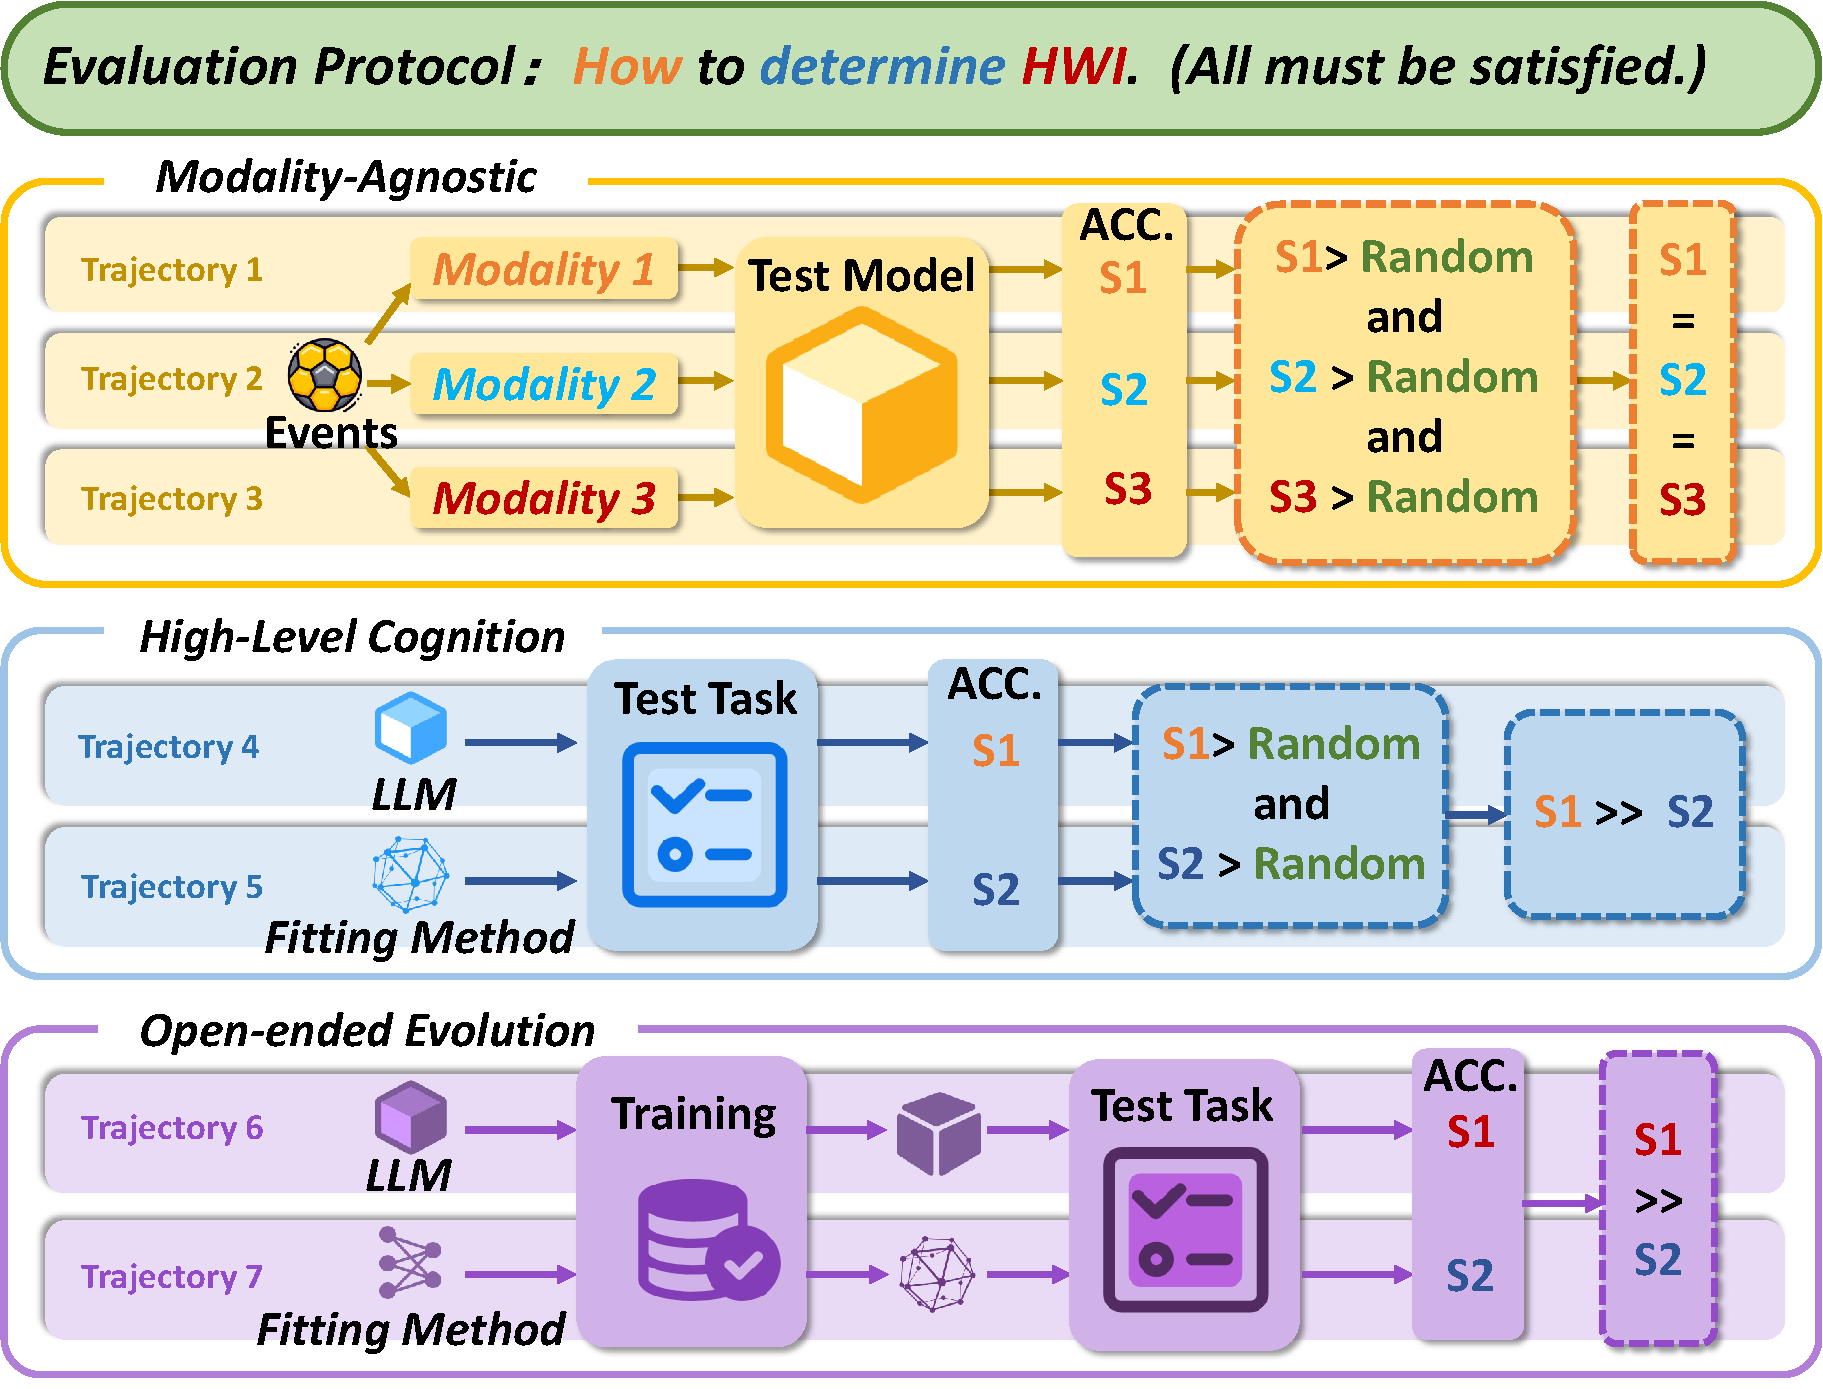
\includegraphics[scale=0.27]{figure/figure21.pdf}
    \vspace{-3mm}
	\caption{Evaluation and Diagnosis pipeline (How to test three capabilities under HWI framework). }
    \vspace{-3mm}
	\label{figure...}
\end{figure}

\subsection{WorldScope Benchmark}
\label{benchmark}

Existing benchmarks predominantly evaluate superficial perception, failing to test models' capacity to \emph{transcend low-level representational barriers} and \emph{formulate high-order macroscopic conclusions}. To address this gap, we introduce \textbf{WorldScope}, a dedicated benchmark for evaluating Holistic World Intelligence, constructing on professional football matches from WhoScored. With the aim at complex physical world characterized by high-dimensional adversarial dynamics, this testbed can rigorously assesses models' HWI capacity boundary. Concretely, WorldScope consists of \emph{two strictly decoupled components} with details in Appendix~\ref{app:construction_pipeline}:
\begin{itemize}[leftmargin=*]
\item \textbf{Low-level Multimodal Input:} We extract fine-grained, fragmented observations for each match, including discrete numerical statistics (e.g., passes, zones), chronological textual commentary, and visual positional heatmaps of all players, while depicting the underlying physical world.
\item \textbf{High-level Integrated Output:} Macroscopic team-style summaries are extracted from various Expert Match Reports and normalized into a finite set of 12 tactical playing styles, which cannot be trivially deduced from isolated foundational data.
\end{itemize}

These strictly decoupled components then perfectly operationalizes our theoretical framework. 
(1) First, by capturing the exact same objective physical event across three heterogeneous channels, the benchmark inherently demands \textbf{Modality-Agnostic} processing, preventing models from exploiting modality-specific semantic shortcuts. 
(2) Furthermore, bridging the representational chasm between raw, fragmented signals and macroscopic tactical labels necessitates genuine \textbf{High-Level Cognition}. Specifically, a model must first perform \textit{understanding} by extracting isolated local features from fragmented inputs (e.g., recognizing discrete passes or shots event from numerical counts, textual commentary, or visual density spots). Next, it must execute \textit{synthesizing} by integrating these scattered events into a coherent global representation (e.g., a panoramic view of the overall match dynamics). Finally, through \textit{reasoning}, it maps this unified representation to high-level conclusions (e.g., deducing macroscopic tactical styles like "favoured short passing"). This process comprehensively forces the model to execute a complete "Understanding-Synthesizing-Reasoning" (U/S/R) cognitive chain. 
(3) Crucially, our continuous real-world football seasons inherently supports \textbf{Open-ended Evolution}. This provides an infinitely renewable environment, allowing models to not only be statically evaluated but also continuously trained to adapt to novel tactical trends, thereby iteratively evolving their alignment with real-world dynamics. 

% Because new matches and expert reports are generated perpetually, the dataset seamlessly scales without the bottleneck of expensive human annotation.
% We curated a substantial dataset of 5,000 matches to ensure robust evaluation. 

As for benchmark's diversity and richness, to mitigate the ambiguity of HWI evaluation, we formulate the testbed into standardized objective tasks: Multiple Choice Questions (MCQ), Single Choice Questions (SCQ), and True/False Questions (TFQ). For consistency, instruction semantics are strictly aligned across all modalities. We also adopt Exact-Match (EM) as accuracy metric after filtering, where any generated content falling outside the finite acceptable ground truth set is categorically penalized as an incorrect response during HWI evaluation.


\begin{table*}[t]
    \centering
    \caption{Comprehensive performance comparison on three modalities (textual, numerical, and visual) and three tasks (MCQ, SCQ, and TFQ). $\dagger$ denotes theoretically calculated values. }
    \vspace{-2mm}
    \label{tab:main_results_hierarchical}
    \renewcommand{\arraystretch}{1.0} 
    \setlength{\tabcolsep}{14pt} % 
    \begin{tabular}{@{} l l c c c c @{}}
        \toprule
        \multirow{2}{*}{\textbf{Category}} & \multirow{2}{*}{\textbf{Model}} & \multirow{2}{*}{\textbf{Params}} & \multicolumn{3}{c}{\textbf{Accuracy (\%)}} \\
        \cmidrule(lr){4-6} 
        & & & \textbf{MCQ} & \textbf{SCQ} & \textbf{TFQ} \\
        \midrule
        
        % ==========================================
        % 基线部分
        % ==========================================
        Baseline & Random-Level & - & 12.95$^\dagger$ & 30.81$^\dagger$ & 56.74$^\dagger$ \\
        \midrule
        
        % ==========================================
        % 文本模态
        % ==========================================
        \rowcolor{blue!10} \multicolumn{6}{c}{\textit{Textual Modality}} \\
        \midrule

        \multirow{6}{*}{General (Zero-Shot)} 
         &  GPT-5.4 \cite{singh2025openai} & - & $\underline{15.00} \pm 3.16$ & $\underline{36.20} \pm 4.87$ & $\underline{54.23} \pm 5.11$ \\
        & Claude-4.6-opus \cite{mukherjee2026red} & - & $14.40 \pm 2.06$ & $33.20 \pm 4.53$ & $53.54 \pm 2.28$ \\
        & Llama-3.1 \cite{grattafiori2024llama} & ~70B & $11.60 \pm 3.26$ & $35.60 \pm 6.62$ & $53.47 \pm 6.30$  \\
        & Mistral-Small-3 \cite{liu2026ministral} & ~24B & $9.00 \pm 4.20$ & $33.60 \pm 5.95$ & $50.89 \pm 3.81$ \\
        & Qwen-2.5 \cite{yang2025qwen3} & ~3B & $\textcolor{blue}{7.20} \pm 2.71$ & $20.80 \pm 5.11$ & $\textcolor{blue}{38.13} \pm 6.72$ \\
        & vicuna-1.5 \cite{zheng2023judging} & ~7B & $8.40 \pm 1.36$ & $\textcolor{blue}{14.60} \pm 1.62$ & $50.00 \pm 0.00$ \\
        \cmidrule(l){2-6} 
        
        \multirow{3}{*}{Traditional Architecture} 
        & \textbf{LSTM} \cite{hochreiter1997long} & ~4.60M &  $20.00 \pm 3.85$ & $\mathbf{\textcolor{red!60!black}{37.20}} \pm 4.07$ & $\mathbf{\textcolor{red!60!black}{61.74}} \pm 2.27$ \\
        & \textbf{MLP} \cite{rumelhart1986learning} & ~3.98M & $17.20 \pm 1.47$ & $ 33.60 \pm 2.24$ & $58.28 \pm 2.77$ \\
        & \textbf{GRU} \cite{cho2014learning} & ~4.44M & $\mathbf{\textcolor{red!60!black}{21.00}} \pm 2.28$ & $ 36.60 \pm 3.79$ & $60.05 \pm 2.26$ \\
        \midrule

        % ==========================================
        % 数字模态
        % ==========================================
        \rowcolor{orange!10} \multicolumn{6}{c}{\textit{Numerical Modality}} \\
        \midrule
        
        \multirow{6}{*}{General (Zero-Shot)} 
        &  GPT-5.4 \cite{singh2025openai} & - & $10.40 \pm 2.94$ & $33.40 \pm 6.89$ & $54.22 \pm 6.22$ \\
        & Claude-4.6-opus \cite{mukherjee2026red} & - & $\underline{14.40} \pm 3.61$ & $\underline{36.40} \pm 8.27$ & $\underline{56.36} \pm 8.92$  \\
        & Llama-3.1 \cite{grattafiori2024llama} & ~70B & $6.40 \pm 2.42$ & $25.40 \pm 5.54$ & $54.21 \pm 8.67$ \\
        & Mistral-Small-3 \cite{liu2026ministral} & ~24B & $\textcolor{blue}{5.80} \pm 2.64$ & $22.40 \pm 4.88$ & $53.03 \pm 4.53$ \\
        & Qwen-2.5 \cite{yang2025qwen3} & ~3B & $6.00 \pm 0.63$ & $24.80 \pm 3.37$ & $\textcolor{blue}{36.84} \pm 5.95$ \\
        & vicuna-1.5 \cite{zheng2023judging} & ~7B & $12.40 \pm 1.74$ & $\textcolor{blue}{13.80} \pm 0.98$ & $50.00 \pm 0.00$ \\
        \cmidrule(l){2-6} 
        
        \multirow{3}{*}{Traditional Architecture} 
        & \textbf{CNN} \cite{lecun1989backpropagation} & ~0.40M & $23.80 \pm 3.31$ & $ 36.80 \pm 4.71$ & $63.38 \pm 5.65$ \\
        & \textbf{MLP} \cite{rumelhart1986learning} & ~0.43M & $\mathbf{\textcolor{red!60!black}{28.40}} \pm 4.22$ & $\mathbf{\textcolor{red!60!black}{38.80}} \pm 6.68$ & $\mathbf{\textcolor{red!60!black}{63.87}} \pm 4.37$ \\
        & \textbf{GRU} \cite{cho2014learning} & ~0.25M & $24.00 \pm 4.82$ & $32.40 \pm 5.78$ & $60.48 \pm 3.48$ \\
        \midrule
        
        % ==========================================
        % 图像模态
        % ==========================================
        \rowcolor{green!10} \multicolumn{6}{c}{\textit{Visual Modality}} \\
        \midrule
        
        \multirow{6}{*}{General (Zero-Shot)} 
        &  GPT-5.4 \cite{singh2025openai} & - & $8.60 \pm 0.49$ & $26.80 \pm 2.56$ & $52.02 \pm 2.39$ \\
        & Claude-4.6-opus \cite{mukherjee2026red} & - & $11.40 \pm 1.36$ & $\underline{30.60} \pm 5.00$ & $\underline{56.59} \pm 3.55$ \\
        &  Llama-3.2-Vision \cite{grattafiori2024llama} & ~90B &  $7.60 \pm 1.36$ & $21.00 \pm 2.28$ & $\textcolor{blue}{32.55} \pm 4.28$  \\
        & Mistral-Small-3.1 \cite{liu2026ministral} & ~24B & $9.00 \pm 3.63$ & $30.20 \pm 4.26$ & $55.00 \pm 1.89$ \\
        & Qwen-2.5-VL \cite{bai2025qwen3} & ~3B & $\underline{12.00} \pm 2.19$ & $14.80 \pm 3.76$ & $49.26 \pm 5.52$ \\
        & LLaVa-1.5 \cite{liu2024improved} & ~7B & $\textcolor{blue}{5.40} \pm 0.49$ & $\textcolor{blue}{13.40} \pm 2.58$ & $50.00 \pm 0.00$  \\
        \cmidrule(l){2-6}
        
        \multirow{3}{*}{Traditional Architecture} 
        & \textbf{ResNet-18} \cite{he2016deep} & ~11.31M & $21.40 \pm 2.58$ & $35.00 \pm 5.40$ & $62.26 \pm 5.33$ \\
        & \textbf{DenseNet-121} \cite{huang2017densely} & ~7.22M & $23.20 \pm 2.79$ & $35.20 \pm 4.71$ & $60.47 \pm 2.26$ \\
        & \textbf{EfficientNet-B0} \cite{tan2019efficientnet} & ~4.34M & $\mathbf{\textcolor{red!60!black}{24.40}} \pm 2.94$ & $\mathbf{\textcolor{red!60!black}{37.60}} \pm 4.72$ & $\mathbf{\textcolor{red!60!black}{63.11}} \pm 1.85$ \\
        
        \bottomrule
    \end{tabular}
    \vspace{-2mm}
\end{table*}



\subsection{Evaluation Protocol}
\label{protocol}

To systematically bridge the empirical results through WorldScope Benchmark with the theoretical foundations under HWI framework, we establish a rigorous evaluation protocol to shift the theoretical perspective to a verifiable sanity check. In this view, the protocol is specifically designed to diagnose quantitatively whether the tested model sufficiently exhibits three formalized attributes of HWI.

1) \textbf{Modality-Agnostic Check:} \emph{Cross-Modality Alignment.} 
To empirically validate the representational equivalence ~\ref{eq1}, we evaluate models independently across numerical ($m_{num}$), textual ($m_{text}$), and visual ($m_{vis}$) modalities for the same split of objective physical events $E$. 
% A model possessing true HWI should yield highly consistent predictive results regardless of the input modality. 
By juxtaposing the performance across heterogeneous input channels, we can measure this modality gap. 
% Crucially, this evaluation must be strictly anchored against a mathematical random baseline. 
% Comparing against random chance is theoretically imperative to establish foundational validity; mere consistency across modalities is mathematically meaningless if the model is systematically hallucinating or guessing. 
% However, exceeding the random baseline is merely a necessary prerequisite, not a sufficient condition. 
To truly prove models' holistic mechanism $\mathcal{F}$ transcending representational barriers, a model must simultaneously satisfy two rigorous criteria: (1) it must significantly exceed the \emph{random baseline} across all modalities, and (2) it must exhibit a \emph{minimized modality gap}.
% Macro-statistical convergence is deceptive if a model correctly predicts disjoint subsets of samples across different modalities. 
In this case, genuine Modality-Agnosticism mandates that for any specific physical event $E_i \in E$, the derived macroscopic truth $y_i$ must remain invariant across $m_{num}$, $m_{text}$, and $m_{vis}$. 
Then, by sanity check on degradation among modalities, a persistent reliance on modality-specific semantic shortcuts is exposed, thereby invalidating any claim of modality-agnostic capability.


2) \textbf{High-Level Cognition Check:} \emph{Statistical Aggregation and Diagnostic Attribution for $f_R \circ f_S \circ f_U$.} 
To quantify a model's capacity to execute the "Understanding-Synthesizing-Reasoning" chain, we introduce a mean-and-standard-deviation ($\mu \pm \sigma$) profiling strategy. 
First, we need to check \emph{whether models are capable of HLC capability}.
In this case, we have mean accuracy $\mu$ serving as the primary indicator of model's absolute capacity to successfully complete the full mapping from fragmented inputs to high-order conclusions as $y = f_R(f_S(f_U(x)))$, while the standard deviation $\sigma$ quantifies the internal stability of this cognitive chain against data variance. 
Here, models are required to surpass the boundary achieved by task-specific traditional-architecture models with passive data-fitting to empirically establish the genuine, intrinsic emergence of HLC.
Futhermore, we need to check \emph{whether models have the intrinsic ability of HLC capability}.
% Because these compact architectures establish a physical upper bound for "passive data-fitting" within a closed data distribution, a massive foundation model that fails to outperform them in a zero-shot setting fundamentally demonstrates an inability to autonomously construct a genuine endogenous reasoning chain.
% If a model's pre-trained, generalized cognitive capacity is inferior to simple statistical interpolation, any claim of possessing High-Level Cognition is entirely invalidated.  
To pinpoint exact structural bottlenecks when this cognition fails, we introduce a diagnostic U/S/R error attribution mechanism in Appendix ~\ref{sec:usrules}). 
This allows us to deconstruct incorrect predictions and identify precisely which specific sub-function—local feature extraction $f_U$, global integration $f_S$, or high-dimensional deduction $f_R$—fractures when processing complex physical signals.

3) \textbf{Open-ended Evolution Check:} \emph{Evolutionary Baselines vs. Superficial Fitting.} 
Our formulation \ref{eq2} mandates that an intelligent agent can autonomously and structurally reshape its internal logic through environmental interaction. 
To investigate this potential, we benchmark general LLMs against two distinct reference points: traditional task-specific supervised models and fully fine-tuned LLMs. 
Here, traditional-architecture models establish a physical upper bound for "passive data-fitting". 
By further evaluating LLMs before and after task-specific fine-tuning, we can diagnose the nature of their learning and evolution capabilities. 
If the fine-tuned LLMs still fail to surpass the traditional-architecture baselines, it constitutes powerful \emph{counter-evidence} indicating that the parameter updates merely resulted in superficial overfitting to task distribution, rather than triggering the genuine, endogenous structural cognitive growth required for true open-ended evolution.